\section{Mazu Overview}

\iffalse
\begin{figure}
\centering
%\begin{minipage}{.45\textwidth}
  \centering
  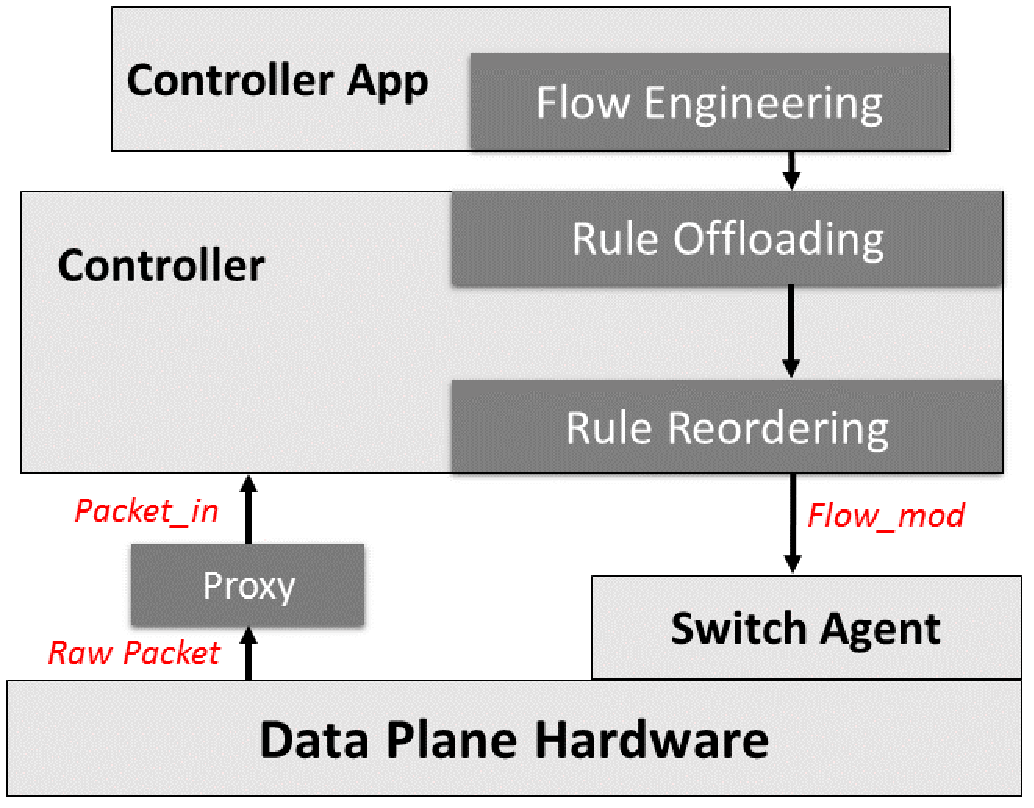
\includegraphics[width=0.25\textwidth]{figs/Mazu_7.pdf}
  %Mazu_frame_new.png}
\caption{Mazu framework}
\label{fig:framework}
\end{figure}
\fi

Our goal is to develop a general set of techniques that an SDN network can
employ to overcome the impact of the latencies described above on key management
applications. Ideally, the techniques must work across all applications,
switches and deployment settings. To this end, we present a new controller framework called Mazu.

%%no packet in story
%To eliminate all inbound delays, and some outbound delays
%(namely, \packetout procesing), we introduce a proxy that generates \packetin
%and processes \packetout messages on behalf of one or more switches.

%The Mazu controller implements a number of modules. The first, i.e., proxy,
%handles inbound processing. We show that the proxy can in fact eliminate all
%inbound delays (\S\ref{s:inbound}). 

Because the underlying causes of outbound delays are tightly linked with
switch software and hardware, we can hope at best to mitigate these
latencies. The remaining modules achieve this. The key insight underlying them
all is to organize the \flowmod\ input provided to switches such that the
aggregate rule installation latency experienced by the application is minimized,
given the underlying latency causes. 

% a framework that 
% previous section on various key management applications. We wish to
% develop a general set of approaches that work across most if not all
% applications and deployment settings. % Our ultimate goal is to ensure
% % applications meet the goals they were designed for as effectively as
% % possible.
% Ideally, the approaches we propose must avoid the latencies altogether. We show that this is possible to achieve for inbound delay. 


% % We present, Mazu, a systematic framework that addresses latency problems
% % comprehensively. 
% % %how a network that has
% % %deployed SDN can overcome the impact of the latencies described in the
% % %previous section on various key management applications. 
% % Our goal is to develop a general set of approaches that work across most if not
% % all applications and deployment settings. 
% %Our ultimate goal is to
% %ensure applications meet the goals they were designed for as
% %effectively as possible.
% As shown in Figure~\ref{fig:framework}, \aditya{not sure we
%   want to show proxy inside the controller, as we argue in the next
%   sectio that this is a bad dea. FIXME}

\iffalse
{\em Flow engineering} is an application-dependent module that computes routes
that spread flows across paths in a network, so as to minimize rule
installation latency by controlling rule displacement at any switch, while
adhering to network objectives (\S\ref{s:floweng}).
{\em Rule offloading} takes the set of rules to be installed at any ingress
switch as an input (these could be rules computed by the flow engineering step
above), and carefully offloads/spreads subsets of these rules to downstream
switches/routers having sufficient capacity to hold the rules
(\S\ref{s:offload}). 
By virtue of reducing the installation latency per switch and enabling parallel 
execution of updates, these techniques ensure rule update tasks finish much
faster.  

% Together these techniques 

% This provides two advantages: (a) it further reduces
% the number of rules installed at any switch. (b) The updates can be
% executed in parallel thereby improving the overall time for insertion.

 {\em Rule Reordering} module reorders the rules to be installed at a
 switch (e.g., those computed by rule offload scheme above) into a
 sequence that is optimal with respect to the switch's hardware table
 management scheme. This helps further control rule installation
 latency (\S\ref{s:optimal}). 


\fi
%This
% techniques mitigates the impact of step 3.

%\aditya{took out multipath probing for now}
%\aditya{cut this out: In multipath probing, the controller sets up multiple
%  paths in parallel so that data plane packets can be 
% switched in hardware as soon as one path completes its setup.  This
% mechanism deals with unexpected delays imposed by switch CPU (e.g.,
% due to CPU  processing
% of other tasks such as polling statistics) and hardware (e.g., due to
% TCAM reorganization). }

% wherein the controller
% probes a collection of otherwise equivalent paths and
% opportunistically installs rules on the path with the lowest likely
% end-to-end installation latency. Whereas the above
% steps apply to proactive batch installation of rules, this step is
% designed for reactive insertion of rules. In such
% situations, paths have to be set up quickly on demand and as such the
% management applications may be unable to control other actions
% switches may be simultaneously executing, such as replying to \pollstats\ or flushing out timed-out rules. \aditya{check this last
%   sentence. also check the font used for the command.}
 
% The multipath probing
% module sets up multiple paths in parallel. Data plane packets can flow through as
% soon as the first path completes installation. This handles variable delay in
% switch updates. The rule offloading module offloads rules to neighboring
% switches to reduce latency. The optimal rule update module tries to update
% switches as fast as it can.
\iffalse
\subsection{Inbound delay}
%We present a novel middlebox that isolates the processing of packet\_in messages
%from other actions on the switch, thereby almost eliminating t\_in. A network
%operator can deploy such middleboxes adjacent to ingress switches in her
%network.
For packet\_in processing, 
To elaborate, a packet typically follows these steps at the switch: 1)
arrives at port and is processed by ASIC, 2) ASIC decides to send "to
CPU" across PCI bus, 3) OS interrupt is raised and ASIC SDK gets
packet, 4) switch-side openflow agent wakes up, processes packet, and
puts on socket to controller.

%a packet typically follows the following steps at the
%switch: 1) arrives at the switch port and PHY, 2) is processed by ASIC, 3) ASIC decides to send "to CPU", 4)
%packet goes across PCI bus to CPU, 5) OS interrupt is raised and handled, 6)
%ASIC SDK gets packet and fires it off to a dispatch hook, 7) switch-side
%openflow agent wakes up, pro- cesses packet, and puts on socket to
%controller. 

Steps 1 to 4 are typically quite fast. The latencies we observe are mainly due to
steps 5 to 7. Earlier measurements show that steps 5 to 7 are slow due to
unoptimized switch implementations. Our measurements indicate that the newer
switches we measured have better implementations of these steps, but latency
arises nevertheless due to contention between simultaneous processing of
packet\_in messages along- side packet\_out flow\_mod and flow statistics
polling messages being received from the controller. 
 
To overcome the inbound latency entirely the key insight we leverage is to
physically decouple the switch's handling of packet\_in and packet\_out messages
from flow\_mod messages. We punt all packet\_in message generation and packet\_out
processing to a separate optimized processing unit, e.g., simple middlebox,
adjacent to the switch. We establish a (short) label-switched path between the
switch and its corresponding middlebox. The switch continues to have a control
channel to the controller (an SSL connection); in addition, we establish a
control channel (SSL) between the middlebox and the controller. The controller
must be aware of the middlebox's presence and must associate it with the
relevant switch. 

To exercise the middlebox, we insert a default low priority rule in the
switch; this helps redirect all unmatched packets on the label-switched path
to the middlebox. The middlebox generates the necessary
packet\_in messages and forwards them on its control channel to the
controller. The controller sends packet\_out messages to the middlebox; the
middlebox process the message and forwards the corresponding data packet to the
switch for further forwarding to the eventual destination. 
%flow\_mod messages directly to the switch. 

\subsection{Outbound delay}
%Ideally, the approaches we propose must avoid the latencies altogether
%to ensure that the applications can be supported effectively. We show
%that this is possible to achieve for inbound delay. However, 
Because
the underlying causes of outbound delays are tightly linked with how
the switches processes and stores forwarding rules, we can hope at
best to mitigate these latencies, and complete avoidance is
impossible. We develop a multi-step approach to maximally mitigate the impact on
outbound delay of various factors we have discovered.

First, we propose flow engineering that attempts to control the aggregate number
of rules inserted at any switch while adhering to the objectives of the
application(s) running. As such, this technique has to be implemented within the
application itself, although, we present a general framework for introducing
flow engineering into a given SDN applications. Flow engineering helps
upper-bound the aggregate impact of steps 1 and 2 above on any given switch. 

Second, we propose rule offload, where a subset of the rules to be installed at
a switch are carefully offloaded to downstream switches/routers having
sufficient capacity to hold the rules. This provides two advantages: (a) it
further reduces the number of rules installed at any switch. (b) The updates can
be executed in parallel thereby improving the overall time for insertion. 

Third, we propose priority ordered insertion, where the rules computed for
insertion at a switch are reordered into a sequence that is optimal with respect
to the switch's hardware table management scheme. This techniques mitigates the impact
of step 3. 

Fourth, for a given flow, we can setup multiple paths in parallel. Data plane
packets can go through as soon as the first path completes setup.
\fi
